\documentclass[12pt]{article}
\usepackage{amsmath}
\usepackage{amssymb}
\usepackage[margin=2.5cm]{geometry}
\usepackage{physics}
\usepackage[hidelinks]{hyperref}
\usepackage[dvipsnames]{xcolor}
\usepackage[indent=12pt]{parskip}
\usepackage{enumitem}
\usepackage{algorithm}
\usepackage{stmaryrd}
\SetSymbolFont{stmry}{bold}{U}{stmry}{m}{n}

\usepackage{booktabs}
\usepackage{algpseudocode} %[noend]
\usepackage{titling}
\usepackage[
    font=small, skip=6pt, labelfont=bf, labelsep=period, 
    format=hang, margin={6pt, 6pt}
]{caption}
\usepackage{graphicx}
% \usepackage{svg}
    
\usepackage{tikz}
\usetikzlibrary{
  calc, patterns, angles, quotes,
  decorations.pathmorphing, decorations.markings, decorations.text,
  shapes, shapes.multipart,backgrounds,arrows.meta,overlay-beamer-styles,
  external
}
\usepackage{epigraph}

\newcommand{\Sin}{%
  \mathop{\sbox0{$\cos$}\makebox[\wd0][r]{$\sin$}}%
}
\newcommand{\SinQ}{%
  \mathop{\sbox0{$\cos^2$}\makebox[\wd0][r]{$\sin^2$}}%
}

\setcounter{tocdepth}{2}
% \setlength{\droptitle}{-3em}
\setlist[itemize]{label=--, itemsep=0pt, topsep=0em}
\setlength{\parskip}{6pt}
\setlength{\parindent}{10pt}

\title{Sun's analemma viewed from earth}
\author{Vincent Degrooff}
\date{\today}

\begin{document}
\maketitle

\setlength{\epigraphwidth}{.45\textwidth}  % ou .9\textwidth
\epigraph{
    Everything is vague to a degree you do not
    realize till you have tried to make it precise
}{Bertrand Russell, \\\textit{The Philosophy of Logical Atomism}}

What is noon? This trivial question hides a reality unsuspected at first glance.
Any sensible person would tell you that noon is when their clock shows 12:00. 
Someone a bit more erudite could answer that noon is when the sun reaches its 
highest point in the sky. Are these two definitions equivalent?

Well, obviously, with the advent of time zones, the answer is no.
But even at Greenwich, located right on the meridian, the two are close but 
do not match! Sometimes by 15 minutes! This is known at least since 
Ptolemy, the Greek astronomer, mathematician and geographer who lived in the 
2nd century.

Let us look in figure \ref{fig:sunrise_sunset} at the sunrise and sunset times 
on the top of \textit{Monte Perdido} in the Pyrenees, located at 42°40'N, 
00°02'E, very close to the meridian. 
Noon is computed as the average of sunrise and sunset times, and as expected, 
it is near 13:00 in winter (CET+1) and near 14:00 in summer (CEST+2). 
But if we zoom in on the data, we see that noon is not constant! It varies by
more than 30 minutes over the year. And this is independent of the latitude!

Defining day length as the time between consecutive noons, we would find that
it is not constant either and by extension, the hours, minutes and 
seconds would change from day to day... This is the definition of 
\textit{apparent solar time}, which is the time measured by a sundial. Low-tech,
but not very practical in our organized society.

Instead, we prefer to use the \textit{mean solar day} which matches the sun's 
average rate of motion over the year. It is simply defined as $86\,400$ seconds,
give or take a few cosmic crumbs that are not our business today.

\begin{figure}[ht]
    \centering
    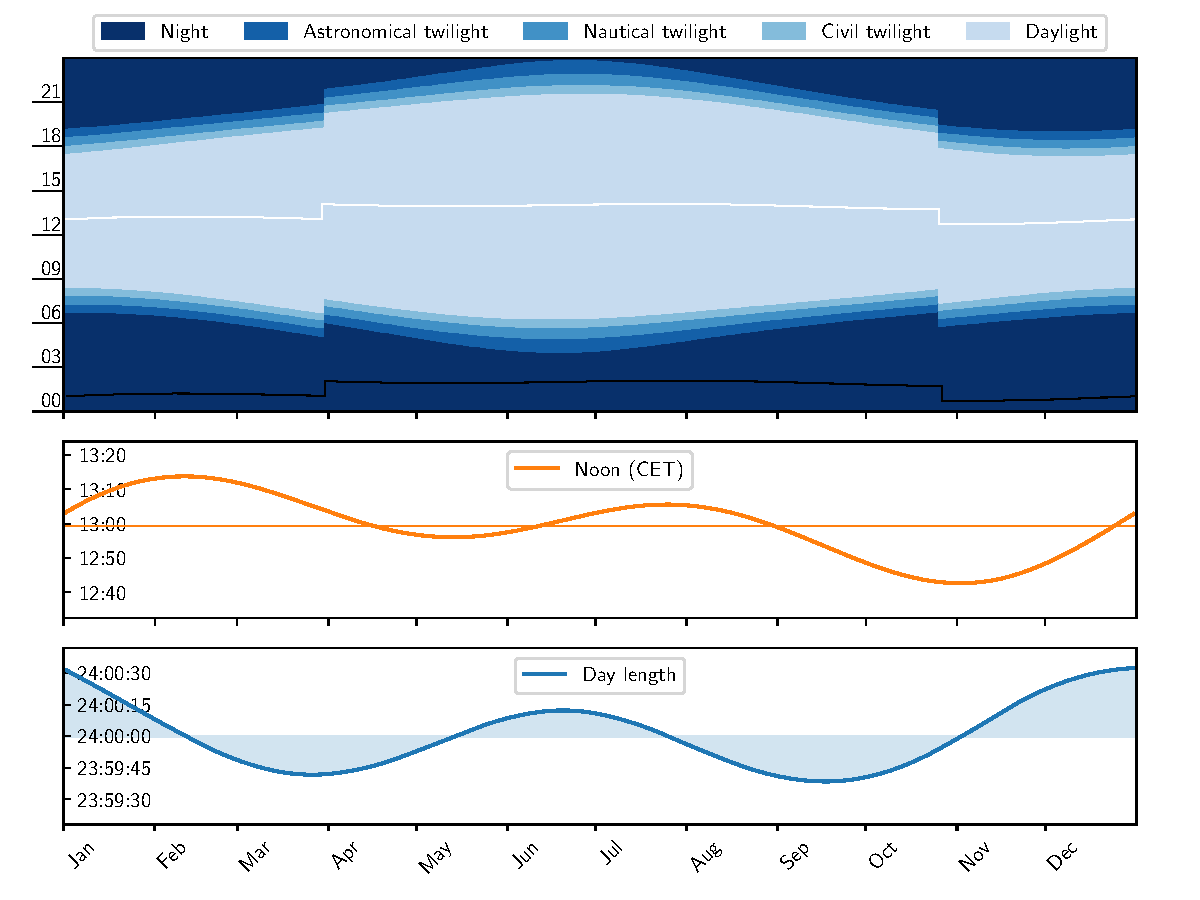
\includegraphics[width=\textwidth]{./sun_graph.pdf}
    \caption{
        Sunrise and sunset times at \textit{Monte Perdido} in local 
        time [data from \texttt{TimeAndDate}].
    }
    \label{fig:sunrise_sunset}
\end{figure}

Then, the natural question is: where is the sun at 12:00 if it is not at its 
highest point? We will answer this question by digging into the math and physics
at play, and discover the beautiful figure drawn by the sun: the analemma.

Someone actually did this experiment and recorded the sun's position
throughout the year 
[\href{https://www.youtube.com/watch?v=Deli5COMJhs}{timelapse link}].


\newpage
The analemma depends on three parameters:
\begin{itemize}
    \item the Earth's axial tilt angle $\epsilon$;
    \item the eccentricity $e$ of the Earth's elliptic orbit;
    \item the argument of periapsis $\omega$, relating the delay 
    from perihelion to spring equinox.
\end{itemize}
To understand why, let's proceed step by step, starting without any of these
parameters.

We should also note that latitude and longitude only translate the analemma
to a different position in the sky, but do not change its shape.

For simplicity, let's furthermore suppose that the year is exactly $N=365$ solar 
days of $T_d = 86400=24\times 60\times 60$ seconds. This is obviously inacurate, 
but sufficent to reveal the beauty of the phenomenon at play.

\clearpage
\section{The simplest case}
\begin{figure}
    \centering
    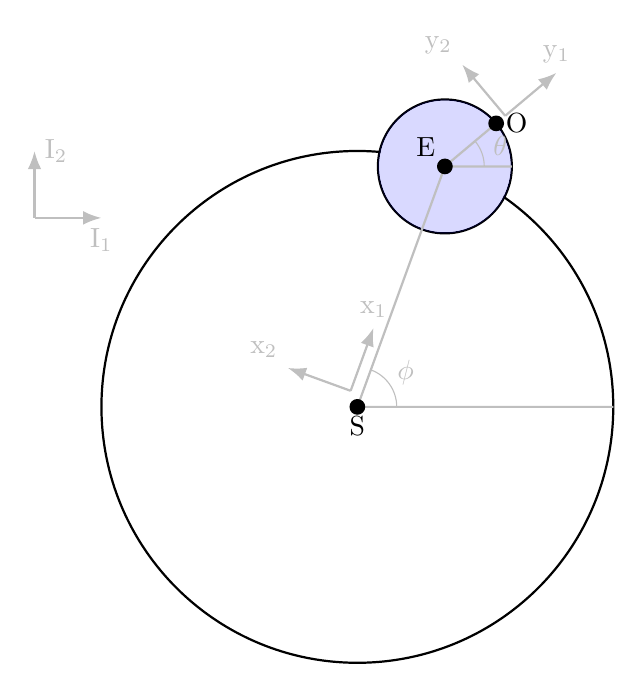
\begin{tikzpicture}
        \pgfmathsetmacro{\rr}{3.25}
        \pgfmathsetmacro{\re}{0.85}
        \pgfmathsetmacro{\ph}{70}
        \pgfmathsetmacro{\th}{40}
        \pgfmathsetmacro{\vv}{0.85}
        \pgfmathsetmacro{\ss}{0.15}
        \pgfmathsetmacro{\bx}{-\rr-\vv}
        \pgfmathsetmacro{\by}{\rr-\vv}
        \coordinate (O) at (0,0);
        \path (O) -- (1,0) coordinate (ex);
        \path (O) -- (0,1) coordinate (ey);
        \path (O) -- (\ph:1) coordinate (u1);
        \path (O) -- ({cos(\ph+90)},{sin(\ph+90)}) coordinate (u2);
        \path (O) -- (\th:1) coordinate (v1);
        \path (O) -- ({cos(\th+90)},{sin(\th+90)}) coordinate (v2);
        \coordinate (A) at (\rr,0);
        \coordinate (E) at ({\rr*cos(\ph)},{\rr*sin(\ph)});
        \coordinate (A0) at ($ (E)!19/20!(O) + \ss*(u2) $);
        \coordinate (A1) at ($ (A0) + \vv*(u1) $);
        \coordinate (A2) at ($ (A0) + \vv*(u2) $);
        \coordinate (S1) at ($ (E) + \re*(ex) $);
        \coordinate (S2) at ($ (E) + \re*(v1) $);
        \coordinate (E0) at ($ (E) + \re*(v1) + \ss*(v1) $);
        \coordinate (E1) at ($ (E0) + \vv*(v1) $);
        \coordinate (E2) at ($ (E0) + \vv*(v2) $);
        \coordinate (B0) at ({\bx}, {\by});
        \coordinate (B1) at ({\bx+\vv}, {\by});
        \coordinate (B2) at ({\bx}, {\by+\vv});
        \draw[thick,-Latex, lightgray] (B0) -- (B1) node[below] {$\mathrm{I}_1$};
        \draw[thick,-Latex, lightgray] (B0) -- (B2) node[right] {$\mathrm{I}_2$};
        \draw[thick,-Latex, lightgray] (A0) -- (A1) node[above] {$\mathrm{x}_1$};
        \draw[thick,-Latex, lightgray] (A0) -- (A2) node[above left] {$\mathrm{x}_2$};
        \draw[thick,-Latex, lightgray] (E0) -- (E1) node[above] {$\mathrm{y}_1$};
        \draw[thick,-Latex, lightgray] (E0) -- (E2) node[above left] {$\mathrm{y}_2$};
        \node at (O) [anchor=north] {S};
        \draw[thick] (O) circle (\rr);
        \draw[thick] (E) circle (\re);
        \fill[color=white] (E) circle (\re*0.98);
        \fill[opacity=0.15, color=Blue] (E) circle (\re);
        \node at (E) [above left] {E};
        \node at (S2) [right] {O};
        \draw[thick,-, lightgray] (S1) -- (E) -- (S2);
        \draw[thick,-, lightgray] (A) -- (O) -- (E);
        \pic [draw, -, "$\theta$", angle eccentricity=1.5, lightgray] {angle = S1--E--S2};
        \pic [draw, -, "$\phi$", angle eccentricity=1.5, lightgray] {angle = A--O--E};
        \fill (O) circle (0.1);
        \fill (S2) circle (0.1);
        \fill (E) circle (0.1);
    \end{tikzpicture}
\end{figure}

The Earth (E) is revolving counterclockwise around the sun (S) in a circular 
orbit of radius $a$, with angular velocity $\dot \phi=\Omega$.
An observer (O) is rotating counterclockwise around the Earth's axis at a 
distance $R$ with angular velocity $\dot \theta$.

The night sky completes a full rotation to an Earth-based observer in just 
under 24 hours. The extra $\sim 4$ minutes account for the fact that, during 
that time, the Earth also moves slightly along its orbit around the sun - by
about $2\pi/N$ radians. As a result, Earth must rotate a bit more for the 
Sun to return to the same position in the sky.

This period is called the \textit{sidereal day}, noted here $T_s$. 
We experience $N$ solar days in a year, but the Earth actually completes $N+1$ 
sidereal days in the same time.
\begin{align}
    \dot\phi = \Omega = \frac{2\pi}{N T_d} \qquad\qquad
    \dot\theta = \frac{2\pi}{T_s} = (N+1) \Omega
\end{align}

We want to find the position of the sun at a given time $t$ in the Earth's 
frame:
\begin{equation}
    \begin{aligned}
        \overrightarrow{OS} &= \overrightarrow{OE} + \overrightarrow{ES}\\
        &= -R \mathrm{y}_1 - a \mathrm{x}_1\\
        &= -R \mathrm{y}_1 - a \Big[\cos(\phi-\theta) \mathrm{y}_1 + \sin(\phi-\theta) \mathrm{y}_2\Big].
    \end{aligned}
\end{equation}
Since $R/a \approx 4\times 10^{-5}$, we will neglect the term $R y_1$.
From here on, we will use the direction vector 
$s\approx \overrightarrow{OS}/\|\overrightarrow{OS}\|$ that neglects
the $R$ term. Rewriting $\phi-\theta$, and expressing 12:00 on day $k$ 
as $t_{k}=T_d/2 + kT_d$, we get:
\begin{align}
    s(t) &= -\Big[\cos(2\pi t/T_d) \mathrm{y}_1 + \sin(2\pi t/T_d) \mathrm{y}_2\Big],\\
    s(t_{k}) &= \mathrm{y}_1.
\end{align}

\section{Effect of Earth's axial tilt}
\begin{figure}
    \centering
    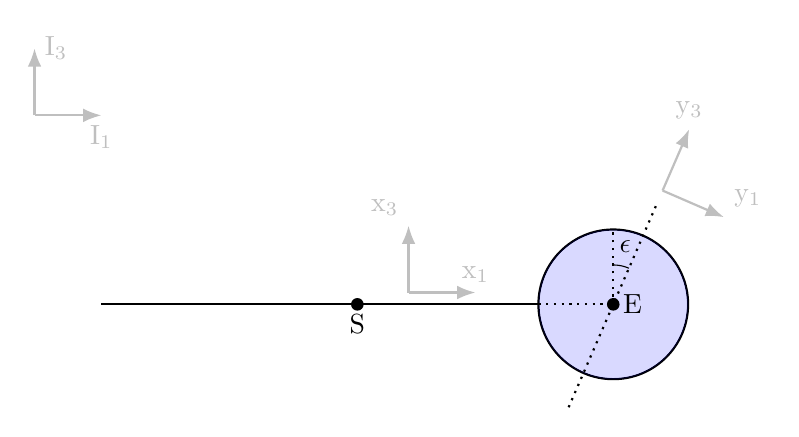
\begin{tikzpicture}
        \pgfmathsetmacro{\rr}{3.25}
        \pgfmathsetmacro{\re}{0.95}
        \pgfmathsetmacro{\ree}{1.5*\re}
        \pgfmathsetmacro{\ph}{70}
        \pgfmathsetmacro{\eps}{23.44}
        \pgfmathsetmacro{\vv}{0.85}
        \pgfmathsetmacro{\ss}{0.15}
        \pgfmathsetmacro{\bx}{-\rr-\vv}
        \pgfmathsetmacro{\by}{\rr-\vv}
        \coordinate (O) at (0,0);
        \path (O) -- (1,0) coordinate (ex);
        \path (O) -- (0,1) coordinate (ey);
        \path (O) -- ({sin(\eps)},{cos(\eps)}) coordinate (u1);
        \path (O) -- ({cos(\eps)},{-sin(\eps)}) coordinate (u2);
        \coordinate (A) at (\rr,0);
        \coordinate (E) at ({\rr},{0});
        \coordinate (A0) at ($ (E)!4/5!(O) + \ss*(ey) $);
        \coordinate (A1) at ($ (A0) + \vv*(ex) $);
        \coordinate (A2) at ($ (A0) + \vv*(ey) $);
        \coordinate (S1) at ($ (E) + \re*(u1) $);
        \coordinate (S2) at ($ (E) + \re*(ey) $);
        \coordinate (E0) at ($ (E) + \ree*(u1) + \ss*(u1) $);
        \coordinate (E1) at ($ (E0) + \vv*(u1) $);
        \coordinate (E2) at ($ (E0) + \vv*(u2) $);
        \coordinate (B0) at ({\bx}, {\by});
        \coordinate (B1) at ({\bx+\vv}, {\by});
        \coordinate (B2) at ({\bx}, {\by+\vv});
        \draw[thick,-Latex, lightgray] (B0) -- (B1) node[below] {$\mathrm{I}_1$};
        \draw[thick,-Latex, lightgray] (B0) -- (B2) node[right] {$\mathrm{I}_3$};
        \draw[thick,-Latex, lightgray] (A0) -- (A1) node[above] {$\mathrm{x}_1$};
        \draw[thick,-Latex, lightgray] (A0) -- (A2) node[above left] {$\mathrm{x}_3$};
        \draw[thick,-Latex, lightgray] (E0) -- (E1) node[above] {$\mathrm{y}_3$};
        \draw[thick,-Latex, lightgray] (E0) -- (E2) node[above right] {$\mathrm{y}_1$};
        \node at (O) [anchor=north] {S};
        \draw[thick] (-\rr, 0) -- (O) -- (E);
        \draw[thick] (E) circle (\re);
        \fill[color=white] (E) circle (\re*0.98);
        \fill[opacity=0.15, color=Blue] (E) circle (\re);
        \node at (E) [right] {E};
        % \node at (S2) [right] {O};
        \draw[thick, dotted] (\rr-\re,0) -- (E);
        \draw[thick, dotted] (E) -- ($ (E) +\re*(ey)$);
        \draw[thick, dotted] ($ (E) -\ree*(u1)$) -- ($ (E) +\ree*(u1)$);
        \pic [draw, -, "$\epsilon$", angle eccentricity=1.5] {angle = S1--E--S2};
        % \draw[thick,-, lightgray] (S1) -- (E) -- (S2);
        % \draw[thick,-, lightgray] (A) -- (O) -- (E);
        % \pic [draw, -, "$\phi$", angle eccentricity=1.5, lightgray] {angle = A--O--E};
        \fill (O) circle (0.08);
        % \fill (S2) circle (0.1);
        \fill (E) circle (0.08);
    \end{tikzpicture}
\end{figure}

The Earth's axis is tilted by an angle $\epsilon=23.44^\circ$ with respect to
the ecliptic plane. The basis $[\mathrm{y}]$ attached to the Earth's frame is 
now obtained after two rotations: first by $\epsilon$ around the $\mathrm{I}_2$ 
axis, then by $\theta$ around the third axis:
\begin{equation}
    \begin{aligned}[c]
        [ \mathrm{y} ] &= R_3(\theta) R_2(\epsilon) [\mathrm{I}] \\
        [ \mathrm{x} ] &= R_3(\phi) R_2(-\epsilon) R_3(-\theta)[\mathrm{y}].
    \end{aligned}
\end{equation}

The sun's position in the Earth's frame $[\mathrm{y}]$ is now given by:
\begin{equation}
    s = -\mathrm{x}_1 =
    \begin{bmatrix}
        -\cos(\phi)\cos(\epsilon)\cos(\theta) - \sin(\phi)\sin(\theta)\\
        \phantom{+}\cos(\phi)\cos(\epsilon)\sin(\theta)-\sin(\phi) \cos(\theta)\\
        -\cos(\phi)\sin(\epsilon)\phantom{\sin(\theta)+\sin(\phi) \cos(\theta)}
    \end{bmatrix}.
    \label{eq:position}
\end{equation}

\textbf{Where is the sun at 12:00?}

Once again, we insert $t_{k}=kT_d+T_d/2$ for $k=0,1,2,\ldots N-1$ in $s$ to 
derive the sun's position at noon. First let's express the angles $\phi$ and 
$\theta$ in terms of $k$:
\begin{equation}
    \left\{
    \begin{aligned}
        \phi &= \Omega t_{k} = 2\pi \frac{1}{N} (k+\tfrac{1}{2})\\
        \theta &= \dot\theta t_{k} = 2\pi \frac{N+1}{N} (k+\tfrac{1}{2})
    \end{aligned}
    \right\} \implies
    \left\{
    \begin{aligned}
        \phi-\theta &= -N\phi = -2\pi (k+\tfrac{1}{2})\\
        \phi+\theta &= (N+2)\phi = 2\pi k + \pi + 2\cdot 2\pi \frac{k+\tfrac{1}{2}}{N}
    \end{aligned}
    \right\}.
\end{equation}

Using trigonometric identities, we find
\begin{equation}
    \begin{aligned}
        \cos(\phi)\cos(\theta)\vert_{12:00} &= -\cos^2\left(2\pi \frac{k+1/2}{N}\right)\\
        \sin(\phi)\sin(\theta)\vert_{12:00} &= -\sin^2\left(2\pi \frac{k+1/2}{N}\right)\\
        \cos(\phi)\sin(\theta)\vert_{12:00} &= -\frac{1}{2} \sin(2\cdot 2\pi \frac{k+1/2}{N})
        = \sin(\phi)\cos(\theta)\vert_{12:00}.
    \end{aligned}
\end{equation}

With these, we can express the analemma as a 
parametric curve with parameter 
$\mu \in [0,2\pi]$:
\begin{equation}
    s\vert_{12:00}(\mu) =
    \frac{1}{2}
    \begin{bmatrix}
        1+\cos\epsilon\\
        0\\
        0
    \end{bmatrix}+
    \frac{1}{2}
    \begin{bmatrix}
        - (1-\cos\epsilon) \cos(2\mu)\\
        \phantom{+} (1-\cos\epsilon) \sin(2\mu)\\
        \quad\;-2\sin(\epsilon) \cos(\phantom{2}\mu)
    \end{bmatrix}.
    % \begin{bmatrix}
    %     \cos(\epsilon)\cos^2(\mu) + \sin^2(\mu)\\
    %     \tfrac{1}{2}(1-\cos(\epsilon)) \sin(2\mu)\\
    %     -\sin(\epsilon) \cos(\mu)
    % \end{bmatrix}.
\end{equation}

This curve is shown in figure \ref{fig:analemma_easy} for various 
tilt angles $\epsilon$, in the observer's frame, that is, without the 
$\mathrm{y}_1$ component. We can note that beyond $\epsilon=90^\circ$, we
enter in a strange territory where the sun is below the horizon at 12:00, with
the day/night cycle reversed.
\begin{figure}[ht]
    \centering
    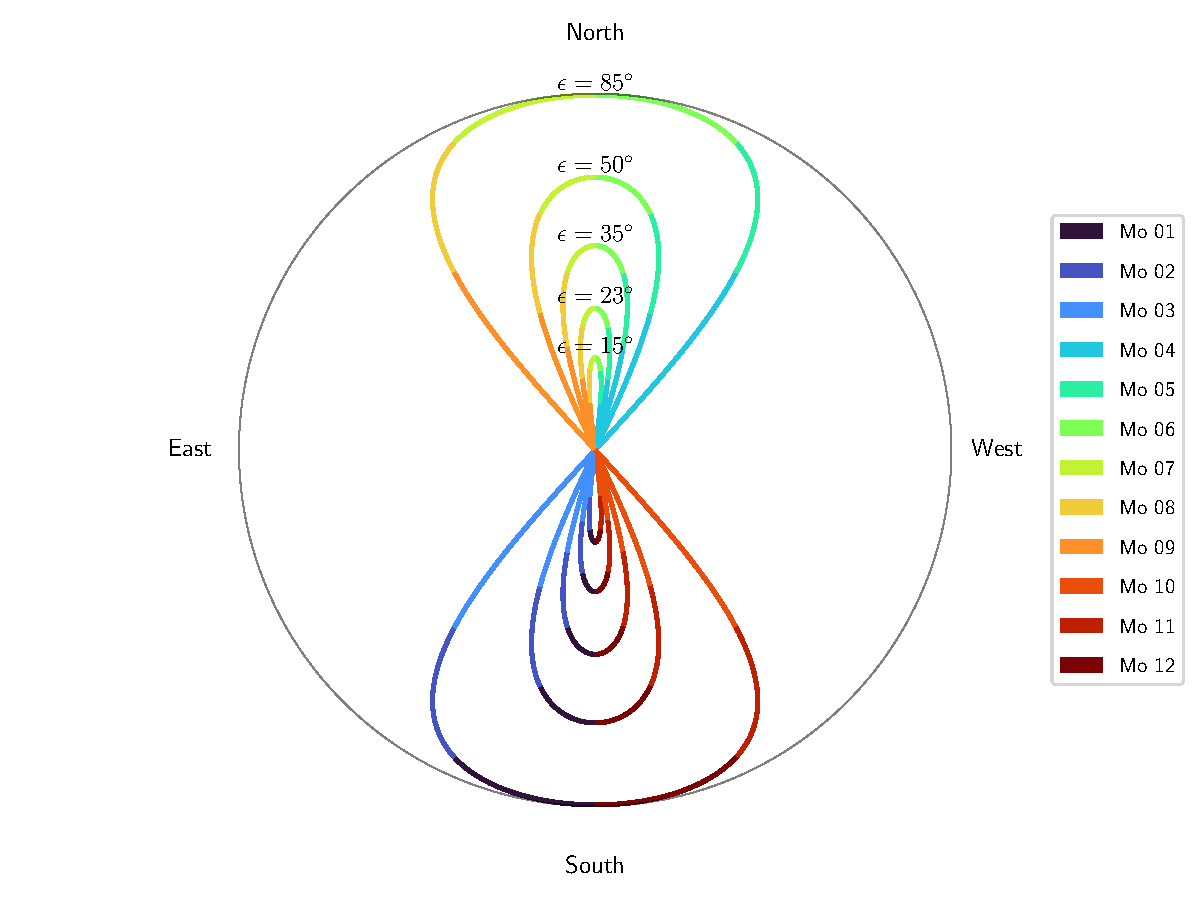
\includegraphics[width=\textwidth]{./analemma_plot.pdf}
    \caption{
        The analemma of 12:00, viewed from the ground at 00°N. 
        The border of the figure is the horizon of the observer. 
        Each month has been assigned a specific color.
    }
    \label{fig:analemma_easy}
\end{figure}


\textbf{When is the sun at its highest point?}

At "solar" noon and midnight, the vector $\mathrm{x}_1$ has no $\mathrm{y}_2$ component:
:
\begin{equation}
    \begin{aligned}
        \cos(\Omega t)\sin\big((N+1)\Omega t\big) \cos(\epsilon) &= \sin(\Omega t) \cos\big((N+1)\Omega t\big)\\
        \iff \quad \sin(N\Omega t)(1-c \cos^2(\Omega t)) &= \frac{c}{2} \cos(N\Omega t) \sin(2\Omega t)
    \end{aligned}
\end{equation}
where $c=1-\cos(\epsilon)$. This equation has no closed form solution for $t^*$,
but we can approximate it around 12:00 with $t^*=kT_d+T_d/2+\delta$, $k=0,1,2\ldots N-1$
:
\begin{equation}
    \left\{
        \begin{aligned}
            \sin(N\Omega t^*) &= -\sin(2\pi\delta / T_d)\\
            \cos(N\Omega t^*) &= -\cos(2\pi\delta / T_d)\\
            \sin(2\Omega t^*) &\approx \sin\big(\tfrac{2\pi}{N} (1+2k)\big)\\
            \cos(\Omega t^*) &\approx \cos\big(\tfrac{\:\pi\:}{N} (1+2k)\big)\\
        \end{aligned}
    \right\} \; \implies \;
    \frac{2\pi \delta}{T_d} \approx \tan(\frac{2\pi \delta}{T_d}) = 
    \frac{c}{2} \frac{\sin(2\cdot 2\pi \tfrac{k+0.5}{N})}{1-c \cos^2(2\pi \tfrac{k+0.5}{N})}.
    \label{eq:noon_shift}
\end{equation}
Noon is off by $\delta$ seconds from the mean solar time, and this shift
oscillates twice a year as we can see with the factor at the numerator of 
\eqref{eq:noon_shift} and in figure \ref{fig:noon_shift}. 
The approximation can be simplified with $\tan(x) \approx x$ 
("approx. 2") and even further by removing the denominator ("approx. 3"),
providing acceptable results until quite large tilt angles $\epsilon$.

\begin{figure}[ht]
    \centering
    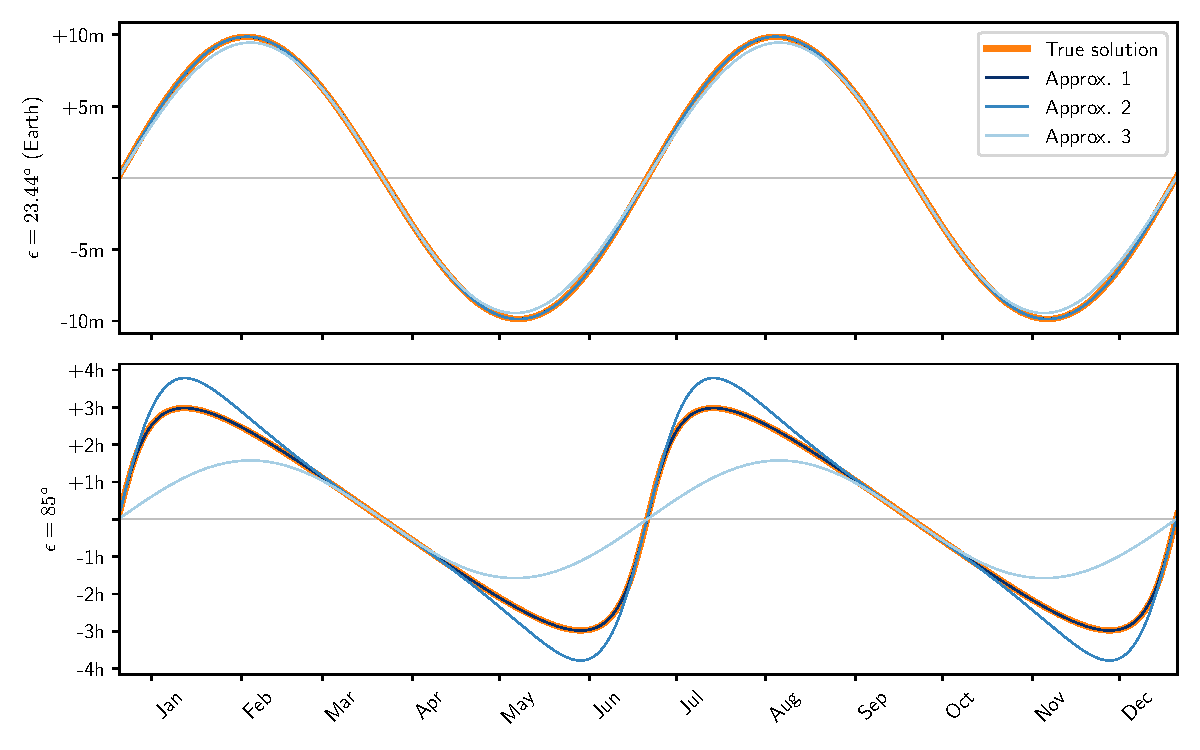
\includegraphics[width=\textwidth]{./noon_computed.pdf}
    \caption{
        Apparent noon time throughout the year for two different axial tilt angles $\epsilon$.
    }
    \label{fig:noon_shift}
\end{figure}

\textbf{An intuitive explanation}

If we consider the Earth's rotating frame,
the sun is revolving around the earth, but also moving up 
(winter and spring) and down (autumn and summer) its equatorial plane.

This vertical motion has a period of one year: the sun reaches its highest point
at the summer solstice, and its lowest point at the winter solstice, for people 
in the northern hemisphere. Since the sun's total motion is constant in this 
cicular orbit model, its horizontal motion must slow down when the vertical 
motion is at its highest \textit{in absolute value}. 

The sun's eastward velocity is thus at its highest
at both solstices, and at its lowest at both equinoxes, producing a
motion of period half a year. This eastward velocity can be observed in 
\ref{fig:noon_shift} as the slope of the apparent noon time. In fact, 
if the sun is moving faster to the East than the average pace, it will take 
more time to reach the zenith, shifting noon a bit later than the day before.

% The sun's horizontal position is simply the
% integral of this velocity as we can see in figure 
% \ref{fig:noon_shift}.

\clearpage
\section{Effect of Earth's orbit eccentricity}

\begin{figure}
    \centering
    \begin{tikzpicture}
        \pgfmathsetmacro{\w}{-8.5}
        \pgfmathsetmacro{\ra}{3.75}
        \pgfmathsetmacro{\rb}{2.8}
        \pgfmathsetmacro{\nnu}{75}
        \pgfmathsetmacro{\gam}{50}
        \pgfmathsetmacro{\vv}{0.85}
        \pgfmathsetmacro{\ss}{0.15}
        \pgfmathsetmacro{\bx}{-\ra/2-1*\vv}
        \pgfmathsetmacro{\by}{0}
        \pgfmathsetmacro{\c}{sqrt(\ra*\ra-\rb*\rb)}
        \pgfmathsetmacro{\e}{\c/\ra}
        \pgfmathsetmacro{\dd}{0.07}
        \pgfmathsetmacro{\cosn}{(cos(\nnu)-\e)/(1-\e*cos(\nnu))}
        \pgfmathsetmacro{\sinn}{(sqrt(1-\e*\e)*sin(\nnu))/(1-\e*cos(\nnu))}
        \pgfmathsetmacro{\mm}{\nnu-\e*sin(\nnu)*180/pi}
        \coordinate (C) at (0,0);
        \coordinate (S) at (\c,0);
        \path (C) -- (1, 0) coordinate (e1);
        \path (C) -- (0, 1) coordinate (e2);
        \path (C) -- ({cos(\gam)},{-sin(\gam)}) coordinate (i1);
        \path (C) -- ({sin(\gam)},{cos(\gam)}) coordinate (i2);
        \path (C) -- ({\cosn},{\sinn}) coordinate (u1);
        \path (C) -- ({-\sinn},{\cosn}) coordinate (u2);
        \coordinate (A) at (\ra,0);
        \coordinate (E) at ({\ra*cos(\nnu)},{\rb*sin(\nnu)});
        \coordinate (EH) at ({\ra*cos(\nnu)},{0});
        \coordinate (EC) at ({\ra*cos(\nnu)},{\ra*sin(\nnu)});
        \coordinate (EM) at ({\ra*cos(\mm)},{\ra*sin(\mm)});
        \coordinate (A0) at ($ (E)!19/20!(S) + \ss*(u2) $);
        \coordinate (A1) at ($ (A0) + \vv*(u1) $);
        \coordinate (A2) at ($ (A0) + \vv*(u2) $);
        \coordinate (B0) at ({\bx}, {\by});
        \coordinate (B1) at ($ (B0) + \vv*(ex) $);
        \coordinate (B2) at ($ (B0) + \vv*(ey) $);
        \coordinate (BH) at ($ (B0) + 2*\vv*(e1) $);
        \fill[blue, opacity=0.1] (S) -- (A) arc(0:\nnu:\ra);
        \fill[orange, opacity=0.1] (O) -- (A) arc(0:\mm:\ra);
        \node at ($(A)-0.0*(ex)$) [anchor=west] {A};
        \node at (C) [anchor=north] {O};
        \node at (S) [anchor=north] {S};
        \draw[thick] (C) ellipse ({\ra} and {\rb});
        \draw[thick, lightgray, dotted] (C) circle ({\ra});
        \draw[thick, lightgray, dotted] (EH) -- (EC);
        \node at (E) [above right] {P};
        \node at (EM) [anchor=west] {P''};
        \node at (EC) [right] {P'};
        \node at (EH) [anchor=north] {D};
        \draw[thick, dotted, lightgray] (S) -- (C) -- (EC);
        \draw[thick, dotted, lightgray] (A) -- (S); 
        \draw[thick, -, lightgray] (S) -- (E) node[pos=0.6, right] {$r$};
        \pic [draw, -, "$\nu$", angle eccentricity=1.5, lightgray] {angle = A--S--E};
        \pic [draw, -, "$E$", angle eccentricity=1.4, lightgray] {angle = A--O--EC};
        \pic [draw, -, "$M$", angle radius=30, angle eccentricity=1.2, lightgray] {angle = A--O--EM};
        % \pic [draw, -, "$\gamma$", angle radius=40, angle eccentricity=1.2, lightgray] {angle = B1--B0--BH};
        \fill (A) circle (\dd);
        \fill (C) circle (\dd);
        \fill (S) circle (\dd);
        \fill (E) circle (\dd);
        \fill (EH) circle (\dd);
        \fill (EM) circle (\dd);
        \fill (EC) circle (\dd);
        % \draw[thick, dotted, lightgray] (B0) -- (BH);
        \draw[thick,-Latex, lightgray] (B0) -- (B1) node[below] {$\mathrm{I}_1$};
        \draw[thick,-Latex, lightgray] (B0) -- (B2) node[right] {$\mathrm{I}_2$};
        \draw[thick,-Latex, lightgray] (A0) -- (A1) node[left=-3pt] {$\mathrm{x}_1$};
        \draw[thick,-Latex, lightgray] (A0) -- (A2) node[below] {$\mathrm{x}_2$};
        %%%%%%%%%%%%%%%%%%%%
        \coordinate (CC) at (\w,0);
        \coordinate (SS) at (\w+\c,0);
        \coordinate (EE) at ({\w+\ra*cos(\nnu)},{\rb*sin(\nnu)});
        \coordinate (AA) at ({\w+\ra}, 0);
        \coordinate (Winter) at (
            {\w+\ra*((cos(-\gam)+\e)/(1+\e*cos(-\gam)))}, 
            {   \rb*(sqrt(1-\e*\e)*sin(-\gam))/(1+\e*cos(-\gam))}
        );
        \coordinate (Spring) at (
            {\w+\ra*((cos(-\gam+90)+\e)/(1+\e*cos(-\gam+90)))}, 
            {   \rb*(sqrt(1-\e*\e)*sin(-\gam+90))/(1+\e*cos(-\gam+90))}
        );
        \coordinate (Summer) at (
            {\w+\ra*((cos(-\gam+180)+\e)/(1+\e*cos(-\gam+180)))}, 
            {   \rb*(sqrt(1-\e*\e)*sin(-\gam+180))/(1+\e*cos(-\gam+180))}
        );
        \coordinate (Autumn) at (
            {\w+\ra*((cos(-\gam+270)+\e)/(1+\e*cos(-\gam+270)))}, 
            {   \rb*(sqrt(1-\e*\e)*sin(-\gam+270))/(1+\e*cos(-\gam+270))}
        );
        \draw[thick] (CC) ellipse ({\ra} and {\rb});
        \draw[dotted] ($ (CC) - \ra*(e1) $) -- (AA);
        \draw[thick, black] (SS) -- (EE);
        \node at (EE) [above right] {P};
        \node at ($ (S) + \w*(e1)$) [below] {S};
        \draw[lightgray] (SS) -- (Winter);
        \draw[lightgray] (SS) -- (Spring);
        \draw[lightgray] (SS) -- (Summer);
        \draw[lightgray] (SS) -- (Autumn);
        \pic [draw, -, "$\nu$", angle radius=10, angle eccentricity=1.6, lightgray] {angle = AA--SS--EE};
        \pic [draw, -, "$\gamma$", angle radius=15, angle eccentricity=1.3, lightgray] {angle = Winter--SS--AA};
        % \pic [draw, -, "$\omega$", angle radius=20, angle eccentricity=1.3, lightgray] {angle = AA--SS--Spring};
        \node at ($ (Winter) + 0.4*(ex) + 0.0*(ey)$) [lightgray, anchor=north, text width=1.1cm, align=center, execute at begin node=\setlength{\baselineskip}{6pt}] {\scriptsize Winter solstice};
        \node at ($ (Spring) + 0.4*(ex) - 0.0*(ey)$) [lightgray, anchor=south, text width=1.1cm, align=center, execute at begin node=\setlength{\baselineskip}{6pt}] {\scriptsize Spring equinox};
        \node at (Summer) [lightgray, anchor=south, text width=1.25cm, align=center, execute at begin node=\setlength{\baselineskip}{6pt}] {\scriptsize Summer solstice};
        \node at (Autumn) [lightgray, anchor=north, text width=1.25cm, align=center, execute at begin node=\setlength{\baselineskip}{6pt}] {\scriptsize Autumn equinox};
        \fill ($ (E) + \w*(e1)$) circle (\dd);
        \fill ($ (S) + \w*(e1)$) circle (\dd);
    \end{tikzpicture}
\end{figure}

The Earth's orbit is not a perfect circle, but an ellipse with semi-major axis
$a$ and semi-minor axis $b$. For the earth, the orbit eccentricity 
$e=\sqrt{1-b^2/a^2}\approx 0.017$ is relatively small, but enough to have a
noticeable effect on the analemma. The eccentricity $e\approx 0.66$ in the 
figure above is exaggerated for clarity.

In the early 17th century, Johannes Kepler stated his famous \textit{laws of
planetary motion}:
\begin{enumerate}
    \item The orbit of a planet is an ellipse with the sun at one focus.
    \item A line segment joining a planet and the sun sweeps out equal areas during
        equal intervals of time.
    \item The square of the orbital period of a planet is proportional to the cube
        of the semi-major axis of its orbit.
\end{enumerate}

\textbf{Anomalies}

To describe efficiently a planet's position along its elliptical orbit at a 
given time, astronomers use three angular parameters called \textit{anomalies} to 
stress the difference with a circular orbit. 

\begin{enumerate}
    \item \textit{True anomaly} $\nu$, the angle between the direction of 
    perihelion and the Earth.
    \item \textit{Eccentric anomaly} $E$, an  auxiliary  angle  used to simplify
    calculations.
    \item \textit{Mean anomaly} $M=\Omega t$, increasing linearly with time.
\end{enumerate}

While $M(t)$ increases linearly, Kepler's second law implies that $\nu(t)$ does not: 
the Earth moves faster near perihelion and slower near aphelion. 
This second law states that the blue and orange areas in the figure above 
are equal:
\begin{align}
    |AOP''| &= |ASP'| = |AOP'| - |OSP'|,\\
    \frac{a^2 M}{2} &= \frac{a^2 E}{2} - \frac{(ae) (a\sin e)}{2},\\
    M &= E - e \sin E \label{eq:keplereq}.
\end{align}
The resulting equation \eqref{eq:keplereq} is known as \textit{Kepler's equation} 
and has no closed form solution for $E$ in terms of $M$. Once the eccentric 
anomaly $E$ has been derived from the mean anomaly $M$, it remains to find the 
true anomaly $\nu$:
\begin{align}
    r &= a(1-e \cos E), \label{eq:r}\\[6pt]
    \cos \nu &= \frac{\cos E - e}{1 - e \cos E}, \label{eq:cosnu}\\[0pt]
    \sin \nu &= \frac{\sqrt{1-e^2} \sin E}{1-e\cos E}, \label{eq:sinnu}\\
    r &= a\: \frac{1-e^2}{1+e \cos \nu}.
\end{align}

The relationships \eqref{eq:r}, \eqref{eq:cosnu} and \eqref{eq:sinnu} 
were respectively derived by:
\begin{gather}
    \begin{aligned}
        r^2 &= \|SD\|^2+ \|DP\|^2 = b^2 \sin^2 E + (ae - a \cos E)^2\\
        &= a^2 \left[(1-e^2) (1-\cos^2 E) + (e^2 - 2e \cos E + \cos^2 E)\right]\\
        &= a^2 \left[ 1 - 2e \cos E + e^2 \cos^2 E\right] = a^2 (1-e \cos E)^2,
    \end{aligned}\\[6pt]
    \begin{aligned}
        \|OD\| + \|DS\| &= \|OS\|\\
        a \cos E - r \cos \nu &= ae\\
        a \cos E - a (1-e \cos E) \cos \nu &= ae,
        % \implies \cos \nu &= \frac{\cos E - e}{1-e \cos E}
    \end{aligned}\\[6pt]
    \begin{aligned}
        \|DP\| = r \sin \nu &= b \sin E\\
        a(1-e\cos E) \sin \nu &= a\sqrt{1-e^2} \sin E.
    \end{aligned}
\end{gather}

The true anomaly can be approximated from the mean anomaly
via a Fourier expansion, but to keep the calculations tractable, we will 
limit ourselves to a first-order expansion:
\begin{align}
    \nu &= M + (2e - \tfrac{1}{4}e^3)\sin(M) + \tfrac{5}{4}e^2 \sin(2M) + 
    \tfrac{13}{12}e^3 \sin(3M) + \mathcal{O}(e^4),\\
    &= M + 2e \sin M + \mathcal{O}(e^2).\label{eq:nu_first_order}
\end{align}

Perihelion ($\nu=0$) and winter solstice do not have to coincide,
even though they are quite close currently for Earth which gets closest to the 
sun in early january. The delay between both events is fixed by introducing 
the angle $\gamma$ between perihelion and the winter solstice.

Note also that the planet is assumed to be at perihelion at $t=0$:
\begin{equation}
    \nu(0) = M(0) = \Omega \cdot 0 = 0.
\end{equation} 

\textbf{Planetocentric longitude of perihelion}

The planetocentric longitude of perihelion $\lambda_p$ is defined as the angle
between the direction of the planet's vernal equinox and the direction of its
perihelion.
Not directly available, this information can however be derived 
from first hand astronimical observations. 
The conventional reference frame of this data, is the equatorial coordinate 
system $\mathrm{I}$, whose 1st-axis points in the direction Earth-Sun-Aries 
constellation and 3rd-axis points towards the Earth's north celestial pole.
The parameters needed are listed below: 

\begin{itemize}
    \item The longitude of ascending node $\Omega$, measuring the angle in the 
        ecliptic plane between reference $x$-axis and the planet's ascending 
        node, i.e. where it crosses the ecliptic from south to north;
    \item The longitude of perihelion $\varpi=\omega+\Omega$, a composed angle 
        where $\omega$ is the argument of perihelion, measuring the angle 
        in the planet's orbital plane between the ascending node and the 
        perihelion;
    \item The planet's orbit inclination $i$, the angle between the ecliptic 
        and the planet's orbital plane;
    \item The planet's axis orientation with respect to the reference frame, 
        with its right ascension $\alpha$ and declination $\delta$.
    \item The Earth's axial tilt, or obliquity $\epsilon_0$, the angle between the ecliptic 
        and the Earth's equatorial plane.
\end{itemize}

The sun-planet position vector $p$ at perihelion and the normal to the ecliptic
plane $n$ determine a basis $(p,q,n)$. This basis and the planet's rotation axis
can be obtained through the following rotations:
\begin{align}
    a &= 
    \begin{bmatrix}
        1 & 0 & 0
    \end{bmatrix}
    R_2(-\delta) R_3(\alpha) [\mathrm{I}],\\
    (p,q,n) &= R_3(\lambda_p) 
    % \underbrace{
        R_3(\omega) R_1(i) R_3(\Omega) R_1(\epsilon_0)
    % }_{v} 
    [\mathrm{I}],
\end{align}
where only $\lambda_p$ is unknown. 
The dot product $n\cdot a$ provides the planet's obliquity $\epsilon$.
The spring equinox is reached when 
the planet's rotation axis is orthogonal to its position vector $p$
$p\cdot a=0$, and oriented such that $q \cdot a<0$. This allows us to find 
the planetocentric longitude of perihelion $\lambda_p$:
\begin{gather}
    v \triangleq R_3(\omega) R_1(i) R_3(\Omega) R_1(\epsilon_0) R_3(-\alpha) R_2(\delta)
    \begin{bmatrix}
        1\\
        0\\
        0
    \end{bmatrix},\\
    \begin{bmatrix}
        \cos \lambda_p & \sin \lambda_p\\
        -\sin \lambda_p & \cos \lambda_p
    \end{bmatrix}
    \begin{bmatrix}
        v_1\\
        v_2
    \end{bmatrix}
    \overset{!}{=}
    \begin{bmatrix}
        0\\
        -\sqrt{v_1^2+v_2^2}
    \end{bmatrix}
    = 
    \begin{bmatrix}
        0\\
        -w
    \end{bmatrix},\\[6pt]
    \implies \quad \cos \lambda_p = -\frac{v_2}{w}, \quad
    \sin \lambda_p = \frac{v_1}{w}.
\end{gather}

With $\lambda_p$ now determined, the angle $\gamma$ follows immediately:
$\gamma = \frac{\pi}{2} - \lambda$. This closes the construction by 
linking the solstitial direction to the orbital geometry.

\pagebreak
\textbf{Where is the sun at 12:00?}

With the elliptical orbit, the basis $[\mathrm{y}]$ must now account for the
position of winter solstice before the Earth's axis obliquity is applied,
while the $[\mathrm{x}]$ basis remains unchanged.
\begin{align}
    [\mathrm{y}] &= R_3(\theta) R_2(\epsilon) R_3(-\gamma) [\mathrm{I}],
    \label{eq:base_y}\\
    [\mathrm{x}] &= R_3(\nu) [\mathrm{I}]\label{eq:base_x}
\end{align}

To account for the rotation $\gamma$, we set an initial angle $\theta_0$.
Even though it does not align $y_1$ with $x_1$ at $t=0$, 
$\theta_0=\gamma$ is our prefered choice as it centers the analemma 
in the East-West direction over the year:
\begin{equation}
    \theta(t)=\theta_0+(N+1)\Omega t= \gamma + (N+1)\Omega t.
\end{equation}

Taking into account the varying distance $r$ of the Earth to the sun from 
equation \eqref{eq:r}, and the expressing $x_1$ in the basis $[\mathrm{y}]$
with equations \eqref{eq:base_y} and \eqref{eq:base_x},
we write the position of the sun in the Earth's frame as:
\begin{equation}
    s = -\frac{r}{a} \mathrm{x}_1 =
    \frac{r}{a}\begin{bmatrix}
        -\cos(\epsilon)\cos(\nu+\gamma)\cos(\theta) - \Sin(\nu+\gamma)\Sin(\theta)\\
        \phantom{+}\cos(\epsilon)\cos(\nu+\gamma)\Sin(\theta)-\Sin(\nu+\gamma) \cos(\theta)\\
        -\sin(\epsilon)\cos(\nu+\gamma)\phantom{\Sin(\theta)+\Sin(\nu+\gamma) \cos(\theta)}
    \end{bmatrix}.
    \label{eq:positionEllipse}
\end{equation}

As both $r$ and $\nu$ depend on the eccentricity, we find the required 
first order approximations:
\begin{align}
    r \cos (\nu+\gamma) &= \cos(M+\gamma) - e\Big[
        2\Sin(M+\gamma) \sin M + \cos(M+\gamma)\cos M
    \Big] + \mathcal{O}(e^2)\\
    r \Sin (\nu+\gamma) &= \Sin(M+\gamma) + e\Big[
        2\cos(M+\gamma) \Sin M - \Sin(M+\gamma)\cos M
    \Big] + \mathcal{O}(e^2)
\end{align}

Let's first recall the expressions for noon, the Earth's angular position 
$\theta$, and let's derive a useful relation for integer multiples of the 
angular position $\mu$:
\begin{align}
    t_k &= k T_d + \tfrac{T_d}{2},\\
    M_k &= \Omega t_k = 2\pi \tfrac{k+1/2}{N},\\
    \theta_k &= (N+1)M_k = \gamma + 2\pi k + \pi + M_k \label{eq:theta_ellipse}.
    % (N+\ell)\Omega t_{k} &= 2\pi k + \pi + \ell \mu_k.
\end{align}

Playing around with the trigonometric identities, we find:
{\small
\begin{align}
    r_k \cos (\nu_k) \cos (\theta_k) &\approx 
        -\cos^2(M+\gamma)
        + \frac{e}{4} \Big[
            2\cos M + 3\cos(M+2\gamma) - \cos(3M+2\gamma)
        \Big],
        \label{eq:coscos}\\
    r_k \Sin (\nu_k) \Sin(\theta_k) &\approx 
        -\SinQ(M+\gamma)
        + \frac{e}{4} \Big[
            2\cos M - 3\cos(M+2\gamma) + \cos(3M+2\gamma)
        \Big],
        \label{eq:sinsin}\\
    r_k \cos (\nu_k) \Sin (\theta_k) &\approx 
        -\frac{1}{2}\Sin(2M+2\gamma)
        + \frac{e}{4} \Big[
            4\Sin M + 3\Sin(M+2\gamma) - \Sin(3M+2\gamma)
        \Big],
        \label{eq:cossin}\\
    r_k \Sin (\nu_k) \cos (\theta_k) &\approx 
        -\frac{1}{2}\Sin(2M+2\gamma)
        - \frac{e}{4} \Big[
            4\Sin M - 3\Sin(M+2\gamma) + \Sin(3M+2\gamma)
        \Big].
        \label{eq:sincos}
\end{align}
}

Inserting the approximations \eqref{eq:coscos}--\eqref{eq:sincos} into
equation \eqref{eq:positionEllipse} allows us to approximate the analemma 
up to first order in $e$ with a curve parametrized by $\mu=M+\gamma, \in [0,2\pi]$:
\begin{align}
    s\vert_{12:00}(\mu) &=
    \frac{1}{2}
    \begin{bmatrix}
        1+\cos\epsilon\\[2pt]
        0\\[2pt]
        0
    \end{bmatrix}+
    \frac{1}{2}
    \begin{bmatrix}
        - (1-\cos\epsilon) \cos(2\mu)\\[2pt]
        \phantom{+} (1-\cos\epsilon) \sin(2\mu)\\[2pt]
        \quad\;-2\sin(\epsilon) \cos(\phantom{2}\mu)
    \end{bmatrix}
    + \frac{e}{4}
    \begin{bmatrix}
        \delta_1\\[2pt]
        \delta_2\\[2pt]
        \delta_3
    \end{bmatrix} + \mathcal{O}(e^2),\\[6pt]
    \begin{bmatrix}
        \delta_1\\[2pt]
        \delta_2\\[2pt]
        \delta_3
    \end{bmatrix} &=
    \begin{bmatrix}
        -2(1+\cos \epsilon) \cos(\mu-\gamma) + (1-\cos \epsilon) \big[
            3\cos(\mu+\gamma) - \cos(3\mu-\gamma)
        \big]\\[2pt]
        \phantom{-}4(1+\cos \epsilon)\textcolor{Red}{\Sin(\mu-\gamma)}
            -(1-\cos \epsilon) \big[
            3\Sin(\mu+\gamma) - \Sin(3\mu-\gamma)
        \big]\\[2pt]
        2\sin \epsilon \big[3\cos \gamma - \cos(2\mu-\gamma)\big]
    \end{bmatrix}
\end{align}

Quite an expression! The terms with a factor $(1-\cos\epsilon)$ or 
$\sin\epsilon$ only slightly modify the analemma's shape for moderate 
tilt angles $\epsilon$. The impact of $\delta_1$ is also quite small
for an observer on Earth as he only sees the analemma's projection on the
celestial sphere, i.e. the second and third components of the normalized
position vector $s$.

Let's first consider the case $\gamma=0$ to measure the effect of the 
Earth's orbit eccentricity without the complication of the perihelion shift.
In that case, the vertical symmetry of the analemma is broken. The term 
$e\Sin\mu$ of $\delta_2$, highlighted in red, tends to push the 
analemma towards the East during the first half of the year and towards the 
West during the second half. 
As a consequence, the analemma's southern loop of winter solstice gets widened, 
while the northern loop of summer solstice gets narrowed. 
This effect is illustrated in figures 
\ref{fig:comparisonEarth} and \ref{fig:comparisonMars}.
The effect would be exactly the opposite if we had $\gamma=\pi$,
that is, if the perihelion was at the summer solstice.

Let's then consider the case $\gamma=\pi/2$. Now, the term $e\sin(\mu-\gamma)$
becomes $-e\cos(\mu)$: it pushes the analemma towards the East during spring 
and summer, and towards the West during autumn and winter.
Therefore, the analemma's northern loop of summer solstice gets shifted
towards the East, while the southern loop of winter solstice gets shifted
towards the West. Both loops then keep their original width.

The situation with arbitrary angles $\gamma$ allows a smooth transition 
between both cases and should just be enjoyed visually in figure \ref{fig:mosaic}. 
There, we observe that the first-order approximation remains highly accurate 
for eccentricity values up to $0.3$.

Until now, we have only considered the analemma at 12:00 on the equator, both
in the mathematical model and in figures \ref{fig:analemma_easy}-\ref{fig:mosaic}. From other latitudes, the 
analemma would appear the same but simply lower in the sky. Earlier in 
the day, the analemma would be rotated lower and eastward, 
while later in the day, it would be rotated lower and westward.

\begin{figure}
    \centering
    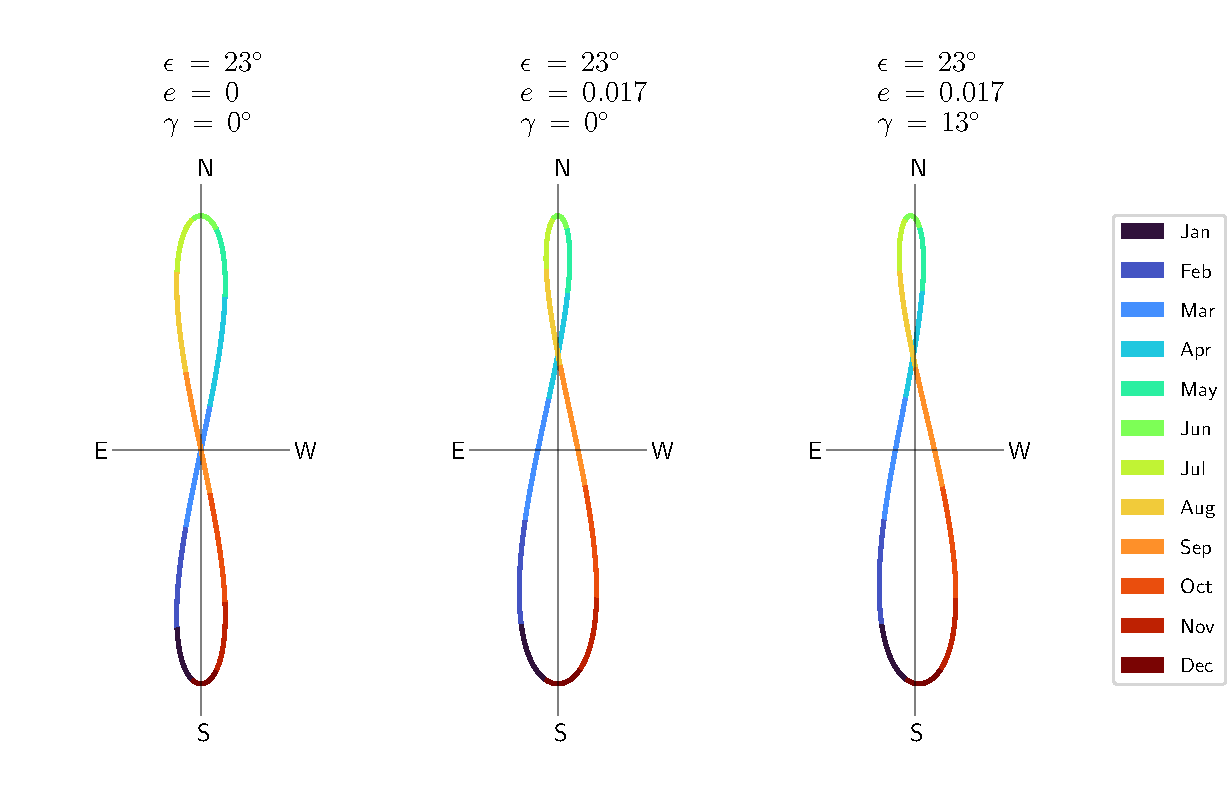
\includegraphics[width=0.92\textwidth]{./comparisonEarth.pdf}
    \caption{
        12:00 Earth analemma, viewed from the ground at 00°N. Introducing the 
        eccentricity breaks vertical symmetry, while perihelion shift 
        $\gamma$ breaks horizontal symmetry.
    }
    \label{fig:comparisonEarth}
\end{figure}

\begin{figure}
    \centering
    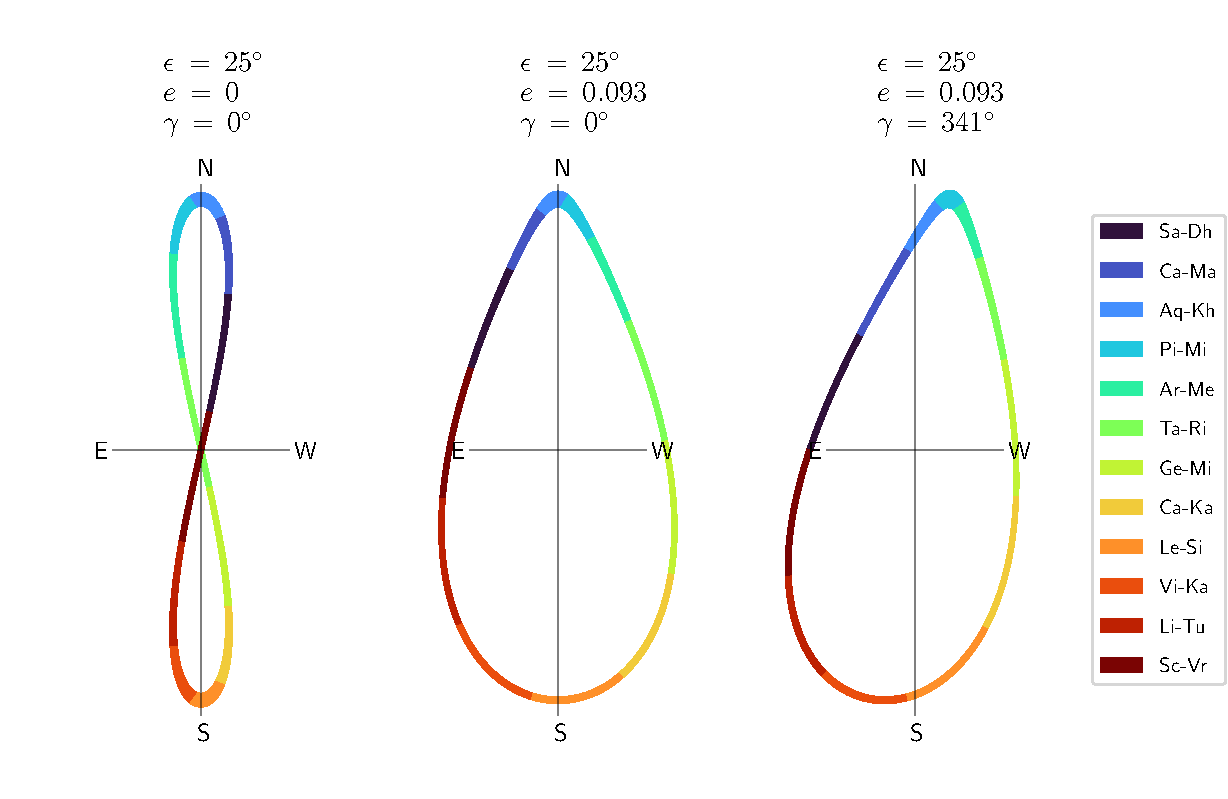
\includegraphics[width=0.92\textwidth]{./comparisonMars.pdf}
    \caption{
        12:00 Mars analemma, viewed from the ground at 00°N. The martian 
        calendar is made of 24 months, grouped here in 6 pairs.
    }
    \label{fig:comparisonMars}
\end{figure}

\begin{figure}
    \centering
    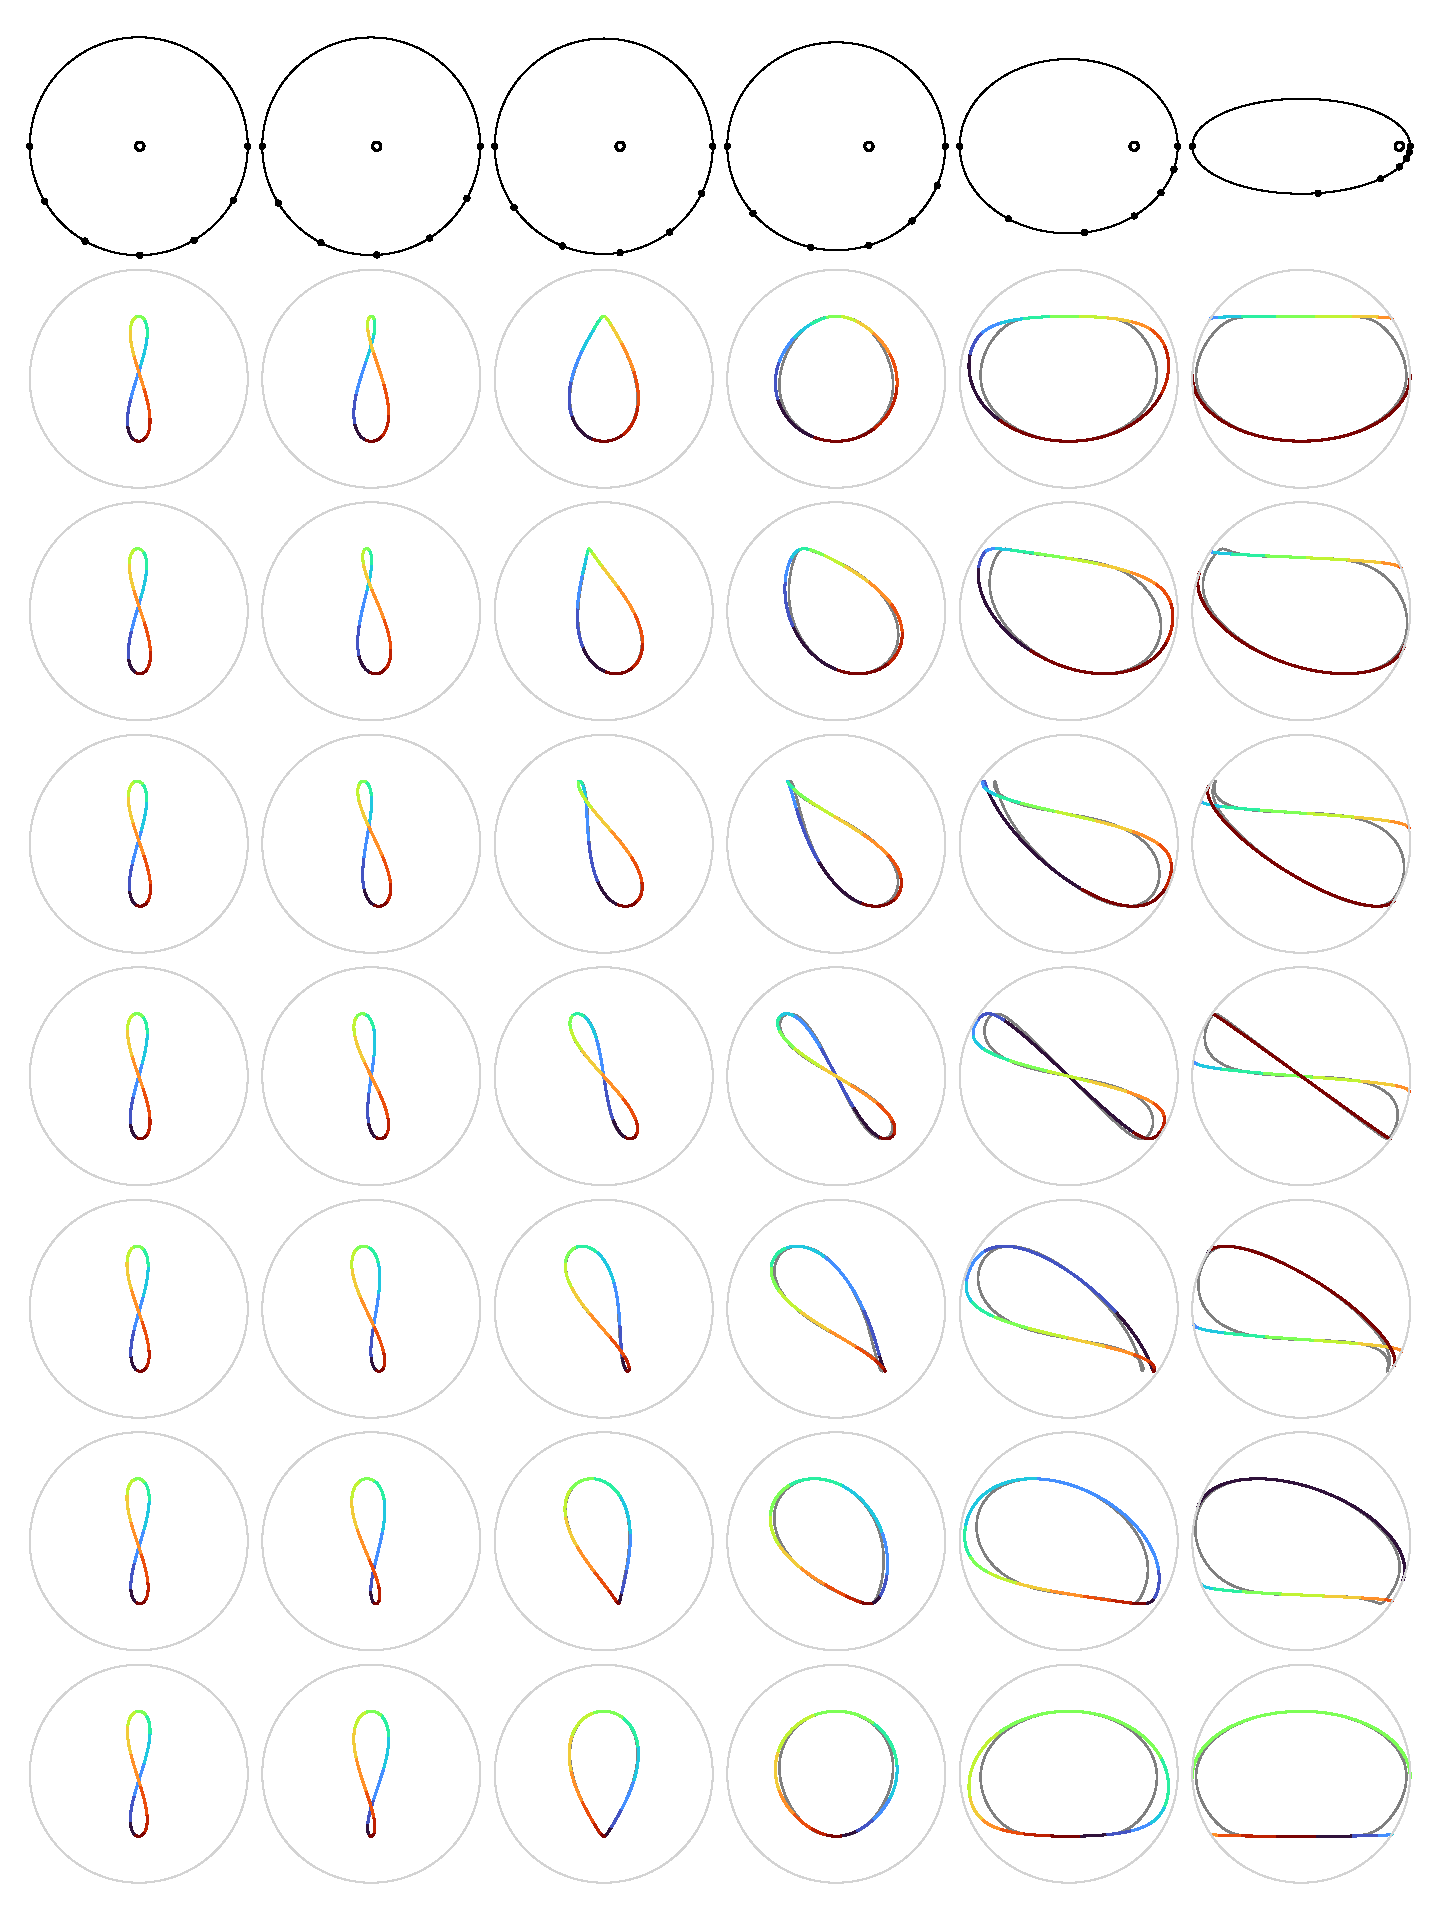
\includegraphics[width=0.98\textwidth]{./mosaic.pdf}
    \caption{
        Noon analemma, viewed from the ground at 00°N, for a tilt angle $\epsilon=35^\circ$, 
        eccentricities $e=0.01, 0.05, 0.15, 0.3, 0.6, 0.9$ and perihelion shifts 
        $\gamma=\tfrac{0\pi}{6},\tfrac{1\pi}{6},\tfrac{2\pi}{6},\tfrac{3\pi}{6},
        \tfrac{4\pi}{6},\tfrac{5\pi}{6},\tfrac{6\pi}{6}$.
    }
    \label{fig:mosaic}
\end{figure}

\pagebreak
\textbf{When is the sun at its highest point?}

Again, at "solar" noon and midnight, the position vector $\mathrm{x}_1$ has no 
component $\mathrm{y}_2$ in the East-West direction. 
Equation \eqref{eq:positionEllipse} gives us the condition
\begin{equation}
    \cos\epsilon \cos(\nu+\gamma) \sin\theta - \sin(\nu+\gamma) \cos\theta = 0,
\end{equation}
where $\nu$ and $\theta$ are functions of time $t$. As said previously, the
true anomaly $\nu$ has no closed form solution, while the rotation angle
$\theta$ is given by equation \eqref{eq:theta_ellipse}. This situation, 
complicated by the eccentricity of the orbit, has obviously no analytical 
solution either.
Let's use our approximation of $\nu$ in equation \eqref{eq:nu_first_order}
% to express $\cos \nu$ and $\sin \nu$ in terms of the shifted mean anomaly 
% $\mu=M+\gamma$:
\begin{equation}
    \begin{aligned}
        \cos \epsilon &\big(
            \cos (M+\gamma) - 2e \Sin(M+\gamma) \Sin M
        \big) \Sin\big(
            \gamma + (N+1)M
        \big)\\
        -&\big(
            \Sin (M+\gamma) + 2e\cos(M+\gamma)\Sin M
        \big) \cos\big(
            \gamma + (N+1)M
        \big) = \mathcal{O}(e^2),
    \end{aligned}
\end{equation}
and expand the high frequency sine/cosine terms to reach, with $\mu=M+\gamma$,
\begin{equation}
    \begin{aligned}
        &\sin(N\Omega t_k) \Big[
            \underbrace{\cos\epsilon \cos^2\mu + \sin^2\mu}_{C} 
            + e \underbrace{
                (1-\cos\epsilon) \sin (\mu-\gamma)\sin 2\mu
            }_D
        \Big] \\
        = &\cos(N\Omega t_k) \Big[
            \underbrace{\tfrac{1-\cos\epsilon}{2} \sin(2\mu)}_A 
            + e \underbrace{
                2\sin(\mu-\gamma) (\cos \epsilon \sin^2 \mu + \cos^2 \mu)
            }_B\Big]
        +\mathcal{O}(e^2).
    \end{aligned}
    \label{eq:noon_time_ellipse}
\end{equation}

We will use the same assumption as in equation \eqref{eq:noon_shift} that the 
time $t^*$ satisfying equation \eqref{eq:noon_time_ellipse} is close to 
noon every day: $t_k=kT_d+T_d/2+\delta_k=M_k+\delta_k$, with 
$k=0,1,2\ldots N-1$ and $\delta_k \ll NT_d$. 
This lets us decouple the periodic terms of low and high frequencies:
\begin{equation}
    \begin{aligned}
        \Sin(N\Omega t_k) &= -\Sin(2\pi\delta_k / T_d)\\
        \cos(N\Omega t_k) &= -\cos(2\pi\delta_k / T_d)\\
    \end{aligned}
    \qquad\qquad
    \begin{aligned}
        \Sin(\ell\Omega t_k) & \approx \Sin(\ell M_k)\\
        \cos(\ell\Omega t_k) & \approx \cos(\ell M_k)
    \end{aligned}
    \qquad
    \text{for } \ell \text{ small}.
    \label{eq:noon_time_approx}
\end{equation}

Introducing the approximations \eqref{eq:noon_time_approx} in equation 
\eqref{eq:noon_time_ellipse}, we can now isolate the time shift $\delta_k$:
\begin{equation}
    \tan(\frac{2\pi \delta_k}{T_d}) 
     = \frac{A+eB}{C+eD} + \mathcal{O}(e^2)
     = \frac{A}{C} + e \frac{B C - A D}{C^2} + \mathcal{O}(e^2).
\end{equation}
After going through some algebra, we finally find an approximation for 
the noon shift $\delta_k$ for a planet with axial tilt $\epsilon$, 
orbit eccentricity $e$ and solstice-perihelion shift $\gamma$ 
on day k with $\mu=\gamma + 2\pi k/N$:
{\small
\begin{equation}
    \tan(\frac{2\pi \delta_k}{T_d})
    = \frac{\tfrac{1}{2}(1-\cos\epsilon)\sin(2\mu)}{1-(1-\cos\epsilon)\cos^2\mu}
        + e \frac{2\cos\epsilon \sin(\mu-\gamma)}{\big[1-(1-\cos\epsilon)\cos^2\mu\big]^2}
    % + e \cos(\epsilon) \frac{2\cos\gamma \sin\mu-\sin\gamma(\cos\mu-\cos3\mu)}{\Big[1-(1-\cos\epsilon)\cos^2\mu\Big]^2}
    +\mathcal{O}(e^2).
\end{equation}
}

This estimate of the noon shift shows us that the shift follows 


\end{document}